

\tikzset{every picture/.style={line width=0.75pt}} %set default line width to 0.75pt        

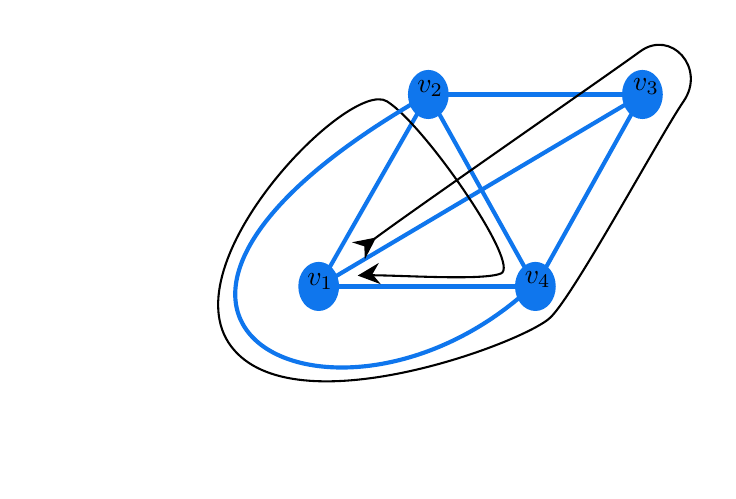
\begin{tikzpicture}[x=0.75pt,y=0.75pt,yscale=-1,xscale=1]
%uncomment if require: \path (0,193); %set diagram left start at 0, and has height of 193

%Shape: Ellipse [id:dp6446268735502532] 
\draw  [draw opacity=0][fill={rgb, 255:red, 15; green, 118; blue, 237 }  ,fill opacity=1 ] (215.97,35.83) .. controls (215.97,29.3) and (220.37,24) .. (225.79,24) .. controls (231.22,24) and (235.61,29.3) .. (235.61,35.83) .. controls (235.61,42.37) and (231.22,47.67) .. (225.79,47.67) .. controls (220.37,47.67) and (215.97,42.37) .. (215.97,35.83) -- cycle ;
%Shape: Ellipse [id:dp5426228859900855] 
\draw  [draw opacity=0][fill={rgb, 255:red, 15; green, 118; blue, 237 }  ,fill opacity=1 ] (164.4,128.32) .. controls (164.4,121.78) and (168.8,116.49) .. (174.22,116.49) .. controls (179.64,116.49) and (184.04,121.78) .. (184.04,128.32) .. controls (184.04,134.86) and (179.64,140.15) .. (174.22,140.15) .. controls (168.8,140.15) and (164.4,134.86) .. (164.4,128.32) -- cycle ;
%Shape: Ellipse [id:dp6391422210469233] 
\draw  [draw opacity=0][fill={rgb, 255:red, 15; green, 118; blue, 237 }  ,fill opacity=1 ] (60,128.32) .. controls (60,121.78) and (64.4,116.49) .. (69.82,116.49) .. controls (75.24,116.49) and (79.64,121.78) .. (79.64,128.32) .. controls (79.64,134.86) and (75.24,140.15) .. (69.82,140.15) .. controls (64.4,140.15) and (60,134.86) .. (60,128.32) -- cycle ;
%Shape: Ellipse [id:dp3528645574747755] 
\draw  [draw opacity=0][fill={rgb, 255:red, 15; green, 118; blue, 237 }  ,fill opacity=1 ] (112.83,35.83) .. controls (112.83,29.3) and (117.23,24) .. (122.65,24) .. controls (128.07,24) and (132.47,29.3) .. (132.47,35.83) .. controls (132.47,42.37) and (128.07,47.67) .. (122.65,47.67) .. controls (117.23,47.67) and (112.83,42.37) .. (112.83,35.83) -- cycle ;
%Straight Lines [id:da495082918303936] 
\draw [color={rgb, 255:red, 15; green, 118; blue, 237 }  ,draw opacity=1 ][line width=1.5]    (174.22,128.32) -- (69.82,128.32) ;
%Straight Lines [id:da5191862136160008] 
\draw [color={rgb, 255:red, 15; green, 118; blue, 237 }  ,draw opacity=1 ][line width=1.5]    (174.22,128.32) -- (122.65,35.83) ;
%Straight Lines [id:da7341802425942472] 
\draw [color={rgb, 255:red, 15; green, 118; blue, 237 }  ,draw opacity=1 ][line width=1.5]    (174.22,128.32) -- (225.79,35.83) ;
%Straight Lines [id:da34230761636576323] 
\draw [color={rgb, 255:red, 15; green, 118; blue, 237 }  ,draw opacity=1 ][line width=1.5]    (69.82,128.32) -- (225.79,35.83) ;
%Straight Lines [id:da2058619078624122] 
\draw [color={rgb, 255:red, 15; green, 118; blue, 237 }  ,draw opacity=1 ][line width=1.5]    (69.82,128.32) -- (122.65,35.83) ;
%Straight Lines [id:da9353037534202] 
\draw [color={rgb, 255:red, 15; green, 118; blue, 237 }  ,draw opacity=1 ][line width=1.5]    (225.79,35.83) -- (122.65,35.83) ;
%Curve Lines [id:da043111183117537255] 
\draw [line width=0.75]    (96.54,105.46) .. controls (117.51,89.9) and (209.84,25.98) .. (224.61,15.15) .. controls (239.61,4.15) and (256.61,23.15) .. (245.61,39.15) .. controls (234.61,55.15) and (193.61,131.15) .. (181.61,143.15) .. controls (169.61,155.15) and (57.61,197.15) .. (27.61,157.15) .. controls (-2.39,117.15) and (84.61,28.09) .. (102.61,39.09) .. controls (120.61,50.09) and (167.61,118.09) .. (157.61,122.09) .. controls (148.31,125.81) and (106.14,122.61) .. (91.44,122.95) ;
\draw [shift={(88.61,123.09)}, rotate = 354.81] [fill={rgb, 255:red, 0; green, 0; blue, 0 }  ][line width=0.08]  [draw opacity=0] (10.72,-5.15) -- (0,0) -- (10.72,5.15) -- (7.12,0) -- cycle    ;
\draw [shift={(97.52,104.74)}, rotate = 503.13] [fill={rgb, 255:red, 0; green, 0; blue, 0 }  ][line width=0.08]  [draw opacity=0] (10.72,-5.15) -- (0,0) -- (10.72,5.15) -- (7.12,0) -- cycle    ;
%Curve Lines [id:da5453842207343367] 
\draw [color={rgb, 255:red, 15; green, 118; blue, 237 }  ,draw opacity=1 ][line width=1.5]    (122.65,35.83) .. controls (-69.39,145.15) and (80.61,216.15) .. (174,127) ;

% Text Node
\draw (62.82,120.72) node [anchor=north west][inner sep=0.75pt]    {$v_{1}$};
% Text Node
\draw (115.82,27.72) node [anchor=north west][inner sep=0.75pt]    {$v_{2}$};
% Text Node
\draw (219.82,26.72) node [anchor=north west][inner sep=0.75pt]    {$v_{3}$};
% Text Node
\draw (167.61,119.55) node [anchor=north west][inner sep=0.75pt]    {$v_{4}$};


\end{tikzpicture}